\textbf{Onderbouw je antwoorden altijd door beredenering en/of berekening.}

Voor een tweefasen PM-stappenmotor is het koppel voor fase A en B:
\begin{align*}
    T_{em,A} &= 6 \cdot i_{s,A} \cdot \sin(4\theta) \, \text{mNm} \\
    T_{em,B} &= 6 \cdot i_{s,B} \cdot \sin(4\theta - 90^\circ) \, \text{mNm}
    \end{align*}\\
Voor volstapbedrijf geldt: \(i_{s,A} = i_{s,B} = 0.5 \, \text{A}\).\\
Men wil met behulp van ministappen extra stappen creeren.    


\begin{enumerate}
    \item [a.] \textbf{Uit hoeveel stappen bestaat 1 omwenteling van de rotor in volstapbedrijf?}
    
        4 stappen om 1 volstap te maken (1 hoek van 90 graden).

    \item [b.] \textbf{Hoeveel ministappen heb je nodig om nullaststanden van $0^\circ ; 2,25^\circ ; 4,5^\circ ; 6,75^\circ ; 9^\circ ; 11,25^\circ$ etc te krijgen?}
    
        $ministappen = \frac{90}{2,25} = 40$

    \item [c.] \textbf{Waarom zal een ministap altijd naar de positie van de nullaststand willen gaan?}
    
        omdat op dit moment geldt $T_{em} = 0$ er staat dan dus geen kracht op de rotor  waardoor hij stil staat.


    \item [d.] \textbf{Kan deze stappenmotor een lastkoppel van 5 mNm verplaatsen?
    Licht je antwoord kort toe.}     
    
        $T_{tot} = T_{em,A} + T_{em,B}$\\
        $T_{em,A} = 6 \cdot i_{s,A} \cdot sin(4 \cdot \theta)$\\
        $T_{em,B} = 6 \cdot i_{s,B} \cdot sin(4 \cdot \theta - 90^\circ)$

        Als je dit voor 1 rondje doet dan krijg je de volgende grafiek:
        \begin{figure}[h]
            \centering
            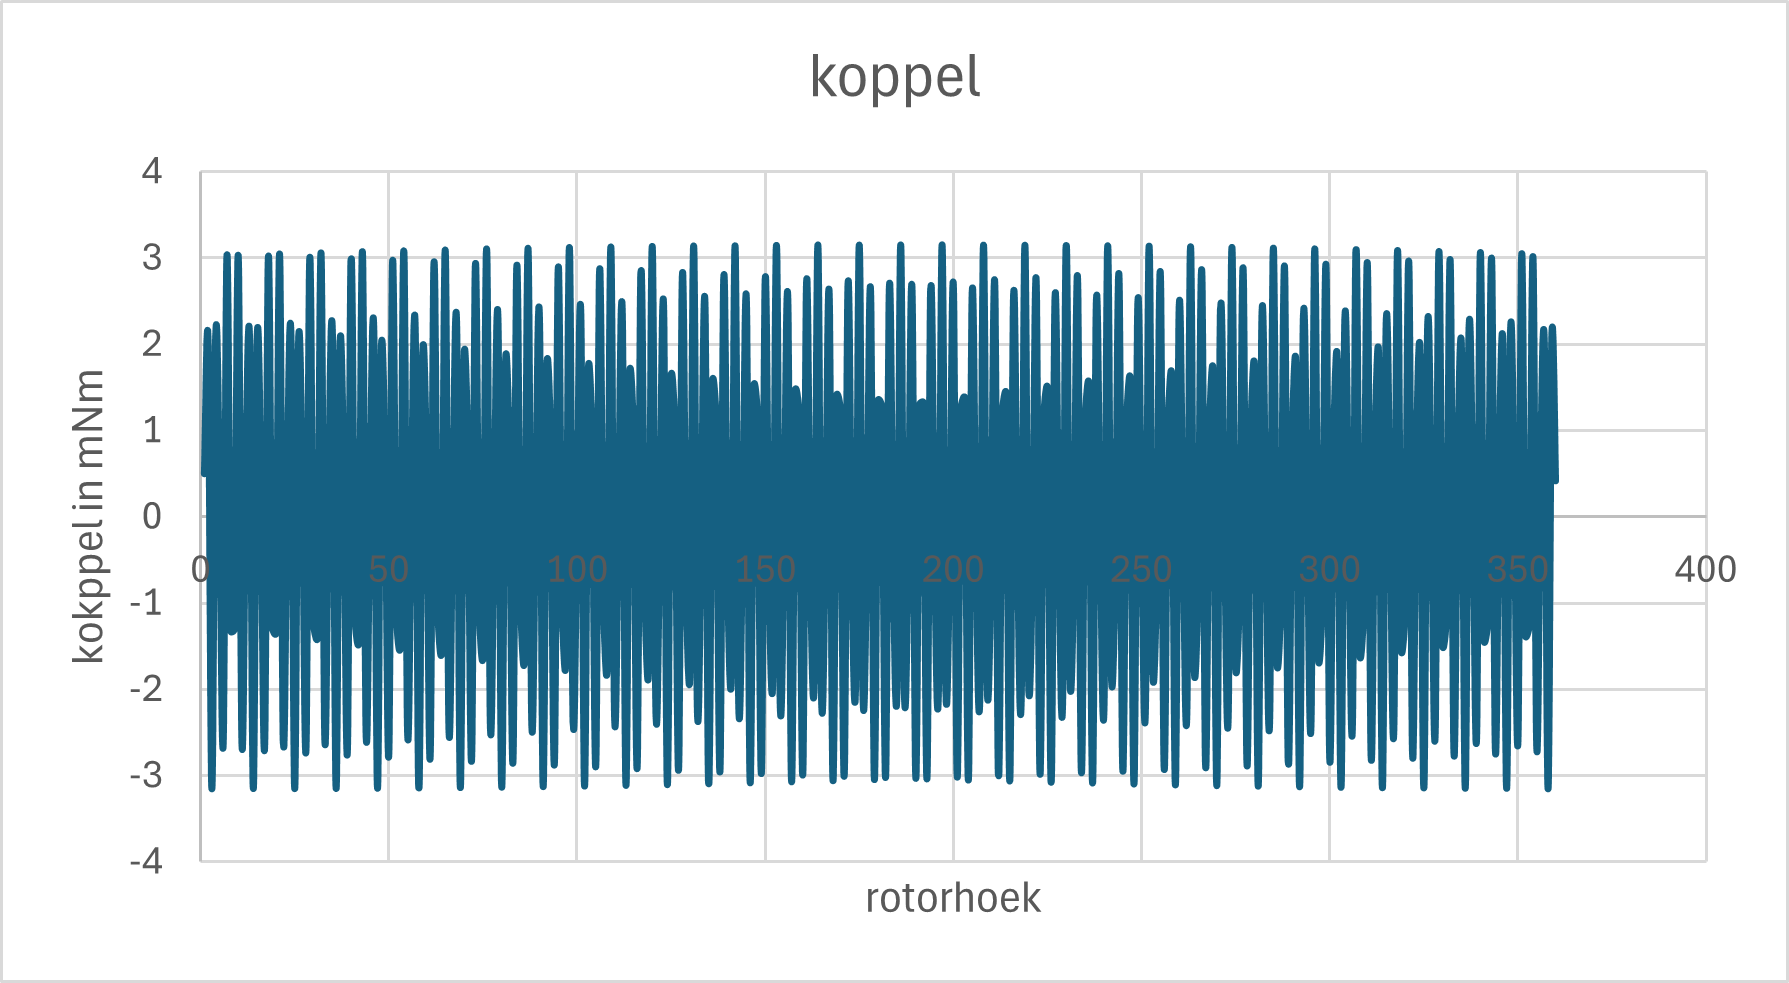
\includegraphics[scale=0.9]{4e.png}
            \caption{koppel}
            \label{fig:4e}
        \end{figure}

        in figuur \ref{fig:4e} is te zien dat de koppel niet echt boven de 3 mNm uit komt en dat het dus niet lukt om 5mNm te verplaatsen.        

    \item [e.] \textbf{Als je bij b) geen antwoord hebt gevonden, ga dan uit van 10 ministappen.
    Hoe groot zijn de stromen $i_{s,A}$ en $i_{s,B}$ om elke afzonderlijke ministap te kunnen
    maken?}
    
        $I_{s,A} = I_{nominaal} \cdot sin(\frac{90}{40} \cdot n) = mA$\\
        $I_{s,B} = I_{nominaal} \cdot cos(\frac{90}{40} \cdot n) = mA$\\
        Waar bij n het aantal microstappen is.

\end{enumerate}